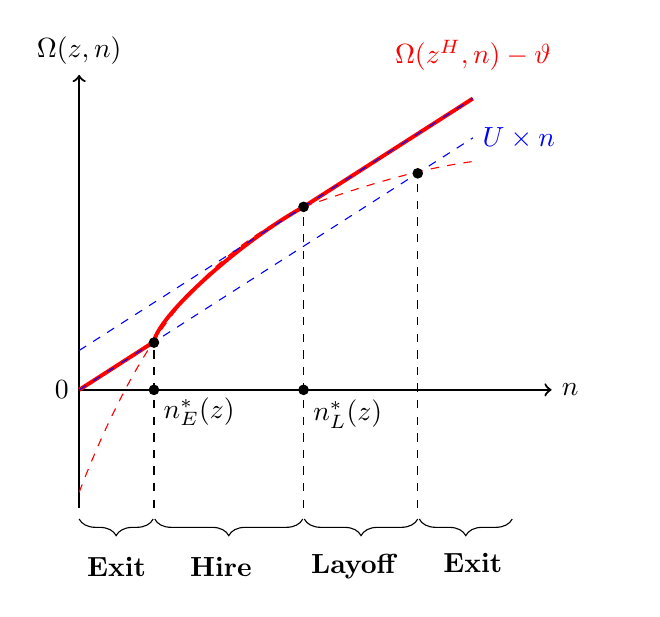
\begin{tikzpicture}

% Axes
\draw[thick,->] (0,0)--(0,5.5) node[above]{$\Omega(z,n)$};
\draw[thick,->] (0,1.5) node[left]{$0$} --(6,1.5) node[right]{$n$};

% Omega
\draw[dashed,red] (0,0.2) ..controls (1,2.8) and (2,3.35) .. (2.85,3.824);
\draw[dashed,red] (2.85,3.824) ..controls (3.5,4.05) and (4.25,4.3) .. (5,4.4);

\draw[line width = 0.5mm,red] (0,1.5)--(0.95,2.11);
\draw[line width = 0.5mm,red] (0.95,2.11) ..controls (1,2.43) and (2,3.35) .. (2.85,3.824);
\draw[line width = 0.5mm,red] (2.85,3.824)--(5,5.2) node[above,yshift=6pt]{$\pmb{\Omega(z^H,n)-\vartheta}$};

% U n
\draw[dashed,blue](0,1.5)--(5,4.7) node[right]{$U \times n$};
\draw[dashed,blue](0,2)--(5,5.2) node[right]{\hskip17.8mm \ };

% Dots
\draw[fill] (0.95,2.1) circle [radius=0.06];
\draw[fill] (2.85,3.824) circle [radius=0.06];
\draw[fill] (4.3, 4.25) circle [radius = 0.06];

% Dashed lines
\draw[dashed] (0.95,0)--(0.95,2.1)node[right,yshift=-25pt]{$n_E^\ast(z)$} ;
\draw[fill]   (0.95,1.5) circle [radius=0.06];
\draw[dashed] (2.85,0) --(2.85,3.824)node[right,yshift=-75pt]{$n_L^\ast(z)$};
\draw[fill]   (2.85,1.5) circle [radius=0.06];
\draw[dashed] (4.3, 0) --(4.3, 4.25);

% Braces
\draw[decorate, decoration = {brace, amplitude = 6pt,mirror}, xshift = 0pt, yshift = -4pt] (0, 0) -- (0.94, 0);
\draw (0.475,-0.75) node{\textbf{\alertroyalblue{Exit}}};

\draw[decorate, decoration = {brace, amplitude = 6pt,mirror}, xshift = 0pt, yshift = -4pt] (0.96, 0) -- (2.84, 0);
\draw (1.8,-0.75) node{\textbf{\alert{Hire}}};

\draw[decorate, decoration = {brace, amplitude = 6pt,mirror}, xshift = 0pt, yshift = -4pt] (2.86, 0) -- (4.3, 0);
\draw (3.5,-0.75) node{\textbf{\alertroyalblue{Layoff}}};

\draw[decorate, decoration = {brace, amplitude = 6pt,mirror}, xshift = 0pt, yshift = -4pt] (4.32, 0) -- (5.5, 0);
\draw (5,-0.7) node{\textbf{\alertroyalblue{Exit}}};

\end{tikzpicture}
